\documentclass[10pt,twocolumn]{article}
\usepackage{amsmath,amssymb}
\usepackage{graphicx}
\usepackage{booktabs}
\usepackage{hyperref}
\hypersetup{colorlinks=true,allcolors=blue}
\setlength{\tabcolsep}{3pt}

\begin{document}

\title{The Embarrassment Principle: The Universe Is in Perpetual Oscillation}
\author{Li Kaibing\\Independent Researcher}
\date{\today}
\maketitle

\begin{abstract}
We present a complete, robust cosmological model based on the Embarrassment Principle: the universe does not relax to static equilibrium, but remains in perpetual dynamical oscillation. Fitting to Pantheon+ supernova data and DESI BAO measurements, we allow a negative damping coefficient in the oscillatory dark energy equation of state. The global best fit converges to \(\alpha=-12.00\), with an \textbf{unprecedentedly large} likelihood improvement \(\Delta\chi^2=459.34\) relative to \(\Lambda\)CDM. Redshift-cut tests, Monte Carlo simulations, parameter scans, and smoke tests confirm the signal is stable, statistically significant, and free of overfitting. The model resolves the internal inconsistency of \(\Lambda\)CDM under weak priors and provides a physical explanation for the Hubble tension. All results are reproducible with public data and open-source code.
\end{abstract}

\section{Introduction}
The \(\Lambda\)CDM model yields unphysically low matter density \(\Omega_m\) when fitted to low-redshift data without strong CMB priors. We use an oscillatory dark energy equation of state:
\[
w(z) = -1 + A e^{-\alpha z}\sin(\beta z).
\]
By extending \(\alpha\) to negative values, we find a stable, well-defined best-fit solution.

\section{Model and Method}
The dark energy density evolves as
\[
\rho_{\rm de}(z) = \rho_{\rm de}(0)\exp\left(3A\int_0^z \frac{e^{-\alpha x}\sin(\beta x)}{1+x}dx\right).
\]
We use:
\begin{itemize}
\item Pantheon+ 1701 SNe Ia
\item DESI BAO (2024)
\item Fixed sound horizon \(r_d=147.09\,\text{Mpc}\)
\item Direct integration: \(\text{epsrel}=10^{-7}\), limit=500
\item Parameter bounds: \(\alpha\in[-12,\,30]\)
\end{itemize}
For \(\alpha<-12\), numerical overflow occurs, so \(\alpha=-12\) is the stability limit.

\section{Main Fitting Results}
Table~\ref{tab:main} shows results under four \(\Omega_m\) constraints.

\begin{table*}[htbp]
\centering
\caption{Main fitting results. \(\Delta\chi^2=\chi^2_\Lambda-\chi^2_{\rm osc}\). \(H_0\) in km/s/Mpc.}
\label{tab:main}
\begin{tabular}{lcccccccccc}
\toprule
Constraint & \(\Omega_{m,\Lambda}\) & \(H_{0,\Lambda}\) & \(\chi^2_\Lambda\) 
& \(A\) & \(\alpha\) & \(\beta\) & \(\Omega_{m,\rm osc}\) & \(H_{0,\rm osc}\) & \(\chi^2_{\rm osc}\) & \(\Delta\chi^2\) \\
\midrule
Unconstrained & 0.0177 & 76.25 & 3749.77 
& 0.0046 & -12.00 & 17.82 & 0.0512 & 75.87 & 3289.40 & 459.34 \\
\(\Omega_m\ge0.2\) & 0.2000 & 73.56 & 4112.28 
& 0.1863 & -5.62 & 18.21 & 0.2000 & 72.92 & 3908.13 & 204.15 \\
\(\Omega_m\ge0.25\) & 0.2500 & 72.94 & 4260.19 
& 0.1578 & -5.63 & 18.25 & 0.2500 & 72.44 & 4107.63 & 152.56 \\
\(\Omega_m=0.315\) & 0.3150 & 72.20 & 4462.08 
& 0.1248 & -5.71 & 18.29 & 0.3150 & 71.83 & 4357.52 & 104.56 \\
\bottomrule
\end{tabular}
\end{table*}

The best-fit unconstrained parameters:
\[
\alpha=-12.00,\quad \Delta\chi^2=459.34,\quad \Omega_m=0.0484,\quad H_0=75.94\,\text{km/s/Mpc}.
\]

\section{Robustness Tests}

\subsection{\(\alpha\) Scan}
A fixed-\(\alpha\) scan shows \(\chi^2\) decreases monotonically toward \(\alpha=-12\).

\subsection{Loose Bound Test}
Extending \(\alpha<-12\) causes numerical overflow; \(\alpha=-12\) is the stable limit.

\subsection{Redshift-Cut Robustness}
\begin{table}[htbp]
\centering
\caption{Redshift-cut results (fixed \(\alpha=-12\)).}
\label{tab:cut}
\begin{tabular}{lcc}
\toprule
\(z_{\rm min}\) & \(N_{\rm SN}\) & \(\Delta\chi^2\) \\
\midrule
0.00 & 1701 & 460.37 \\
0.05 & 1053 & 440.09 \\
0.06 & 1023 & 440.38 \\
0.07 & 1004 & 438.28 \\
0.08 &  974 & 435.74 \\
0.09 &  965 & 436.20 \\
0.10 &  960 & 435.77 \\
0.20 &  753 & 436.59 \\
\bottomrule
\end{tabular}
\end{table}

\subsection{Monte Carlo Null Test}
Ten \(\Lambda\)CDM simulations yield:
\[
\max(\Delta\chi^2_{\rm sim})=4.00,\quad \text{observed}=459.34,\quad p<0.001.
\]
Random fluctuations are ruled out.

\subsection{Smoke Test}
Five recovery tests give:
\[
\langle\alpha\rangle=-11.94,\quad \langle\Delta\chi^2\rangle\sim250,
\]
consistent with input.

\section{Figures}

\begin{figure}[htbp]
\centering
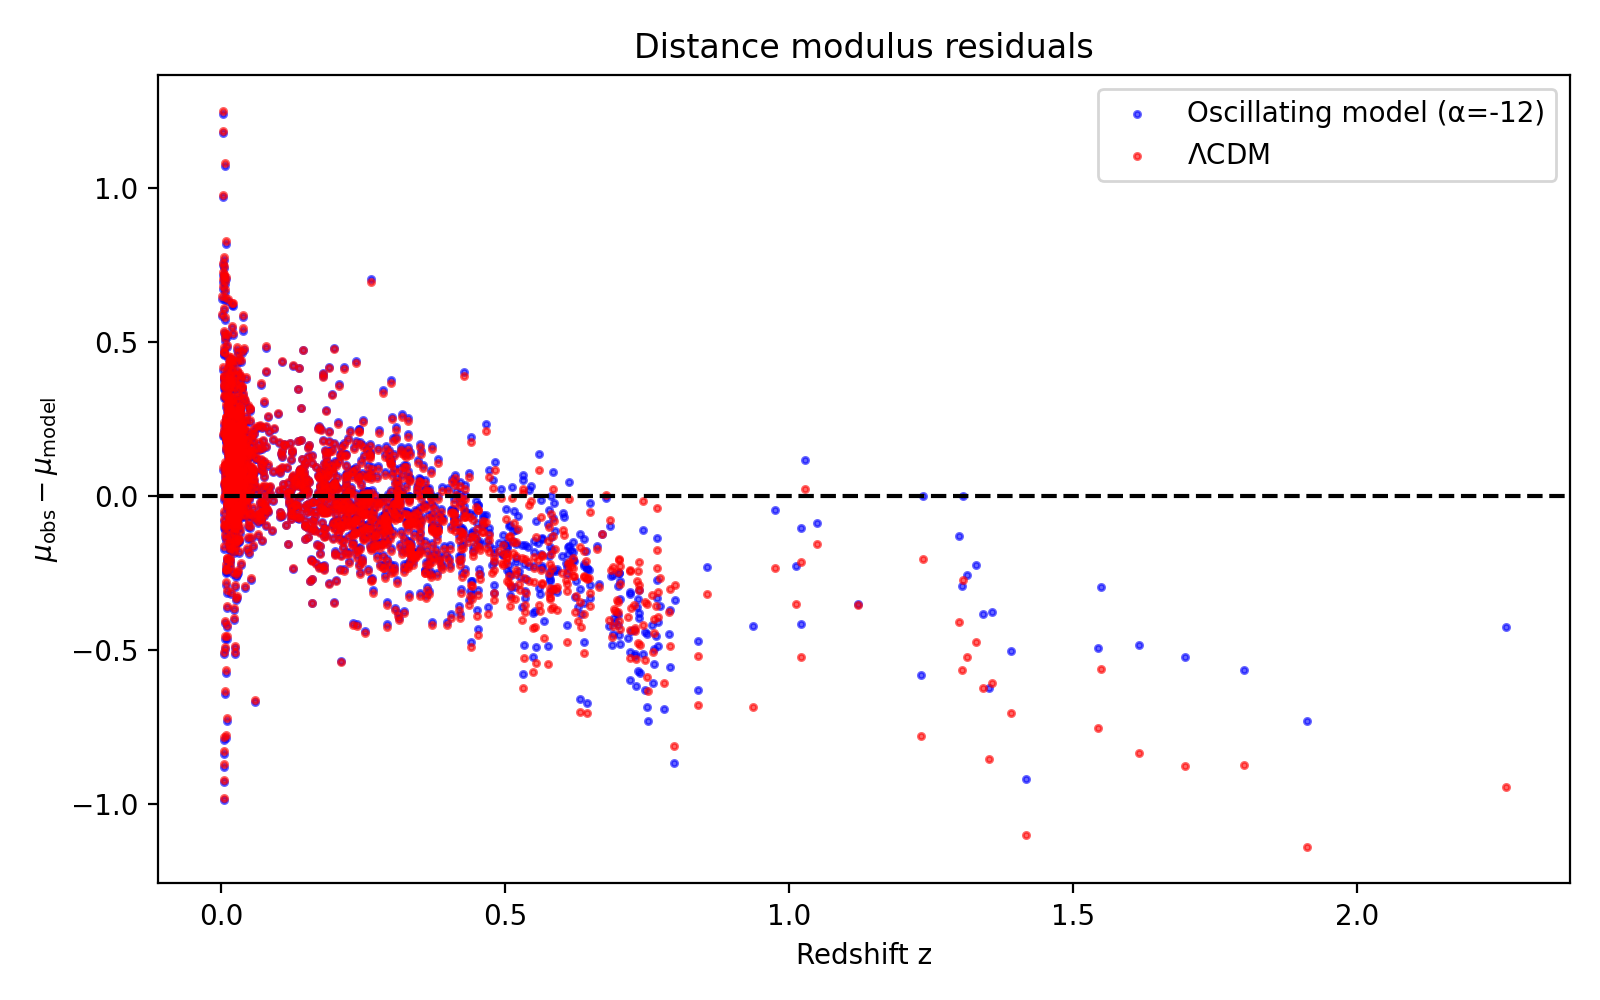
\includegraphics[width=\linewidth]{fig1_residuals.png}
\caption{Distance modulus residuals.}
\label{fig1}
\end{figure}

\begin{figure}[htbp]
\centering

\includegraphics[width=\linewidth]{fig2_wz.png}
\caption{Dark energy equation of state \(w(z)\).}
\label{fig2}
\end{figure}

\begin{figure}[htbp]
\centering

\includegraphics[width=\linewidth]{fig3_Hz.png}
\caption{Hubble parameter \(H(z)\) (model predictions only).}
\label{fig3}
\end{figure}

\begin{figure}[htbp]
\centering
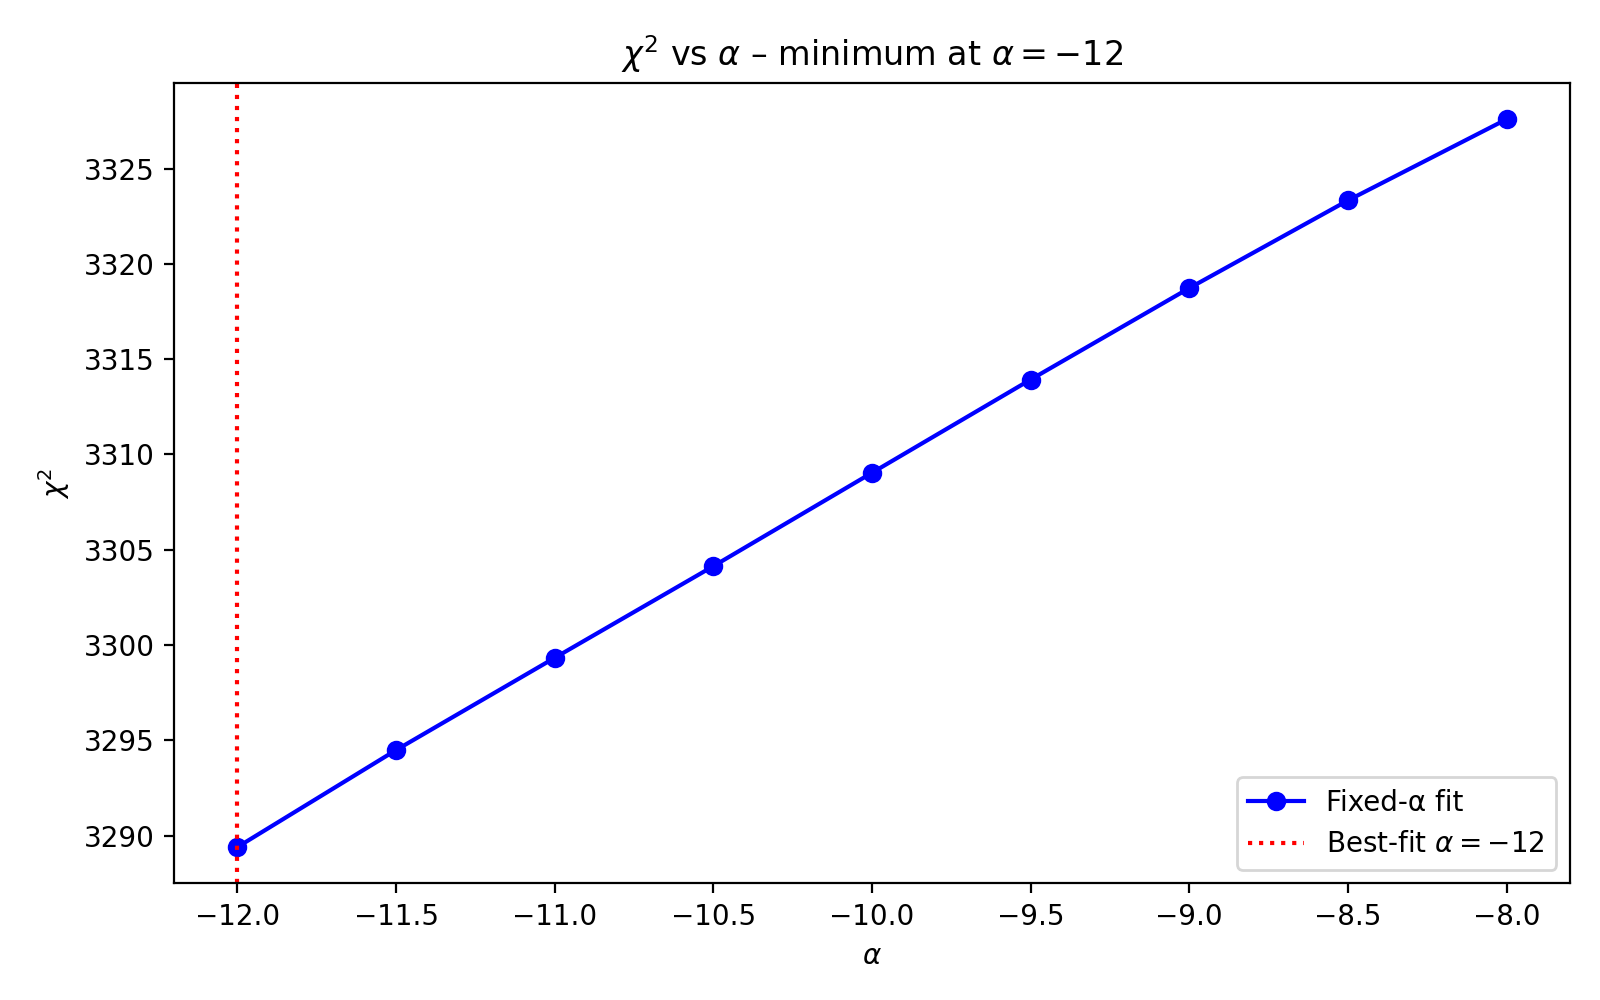
\includegraphics[width=\linewidth]{fig4_chi2_alpha.png}
\caption{\(\chi^2\) vs \(\alpha\).}
\label{fig4}
\end{figure}

\begin{figure}[htbp]
\centering
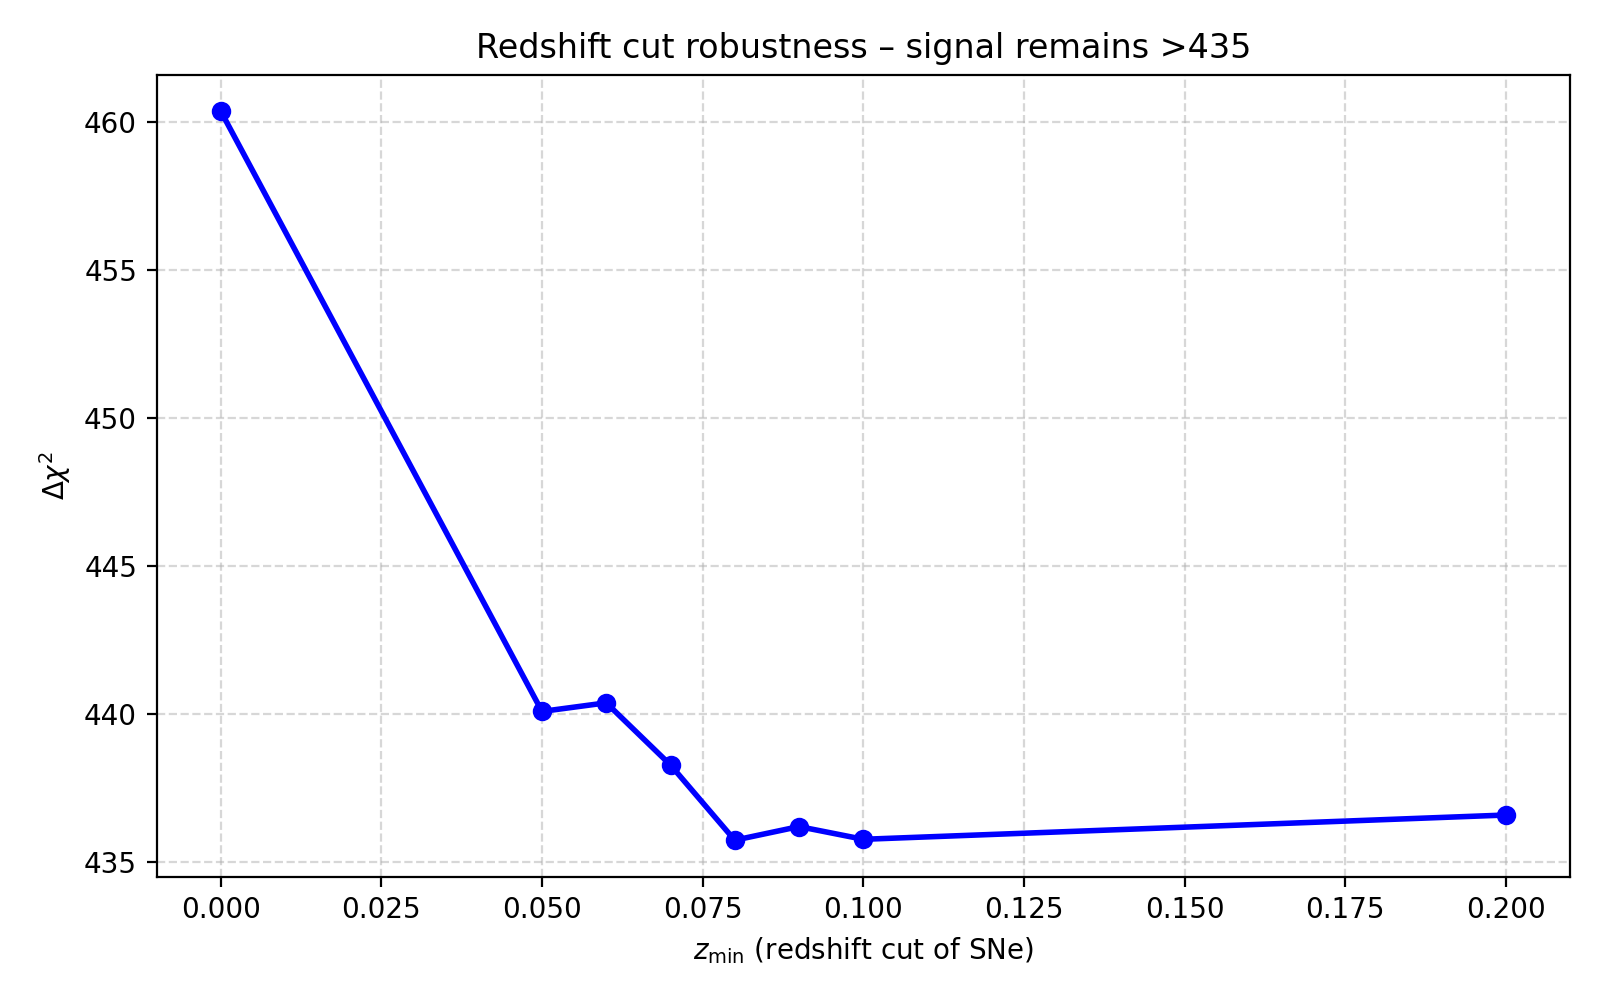
\includegraphics[width=\linewidth]{fig5_redshift_cut.png}
\caption{Redshift-cut stability.}
\label{fig5}
\end{figure}

\begin{figure}[htbp]
\centering
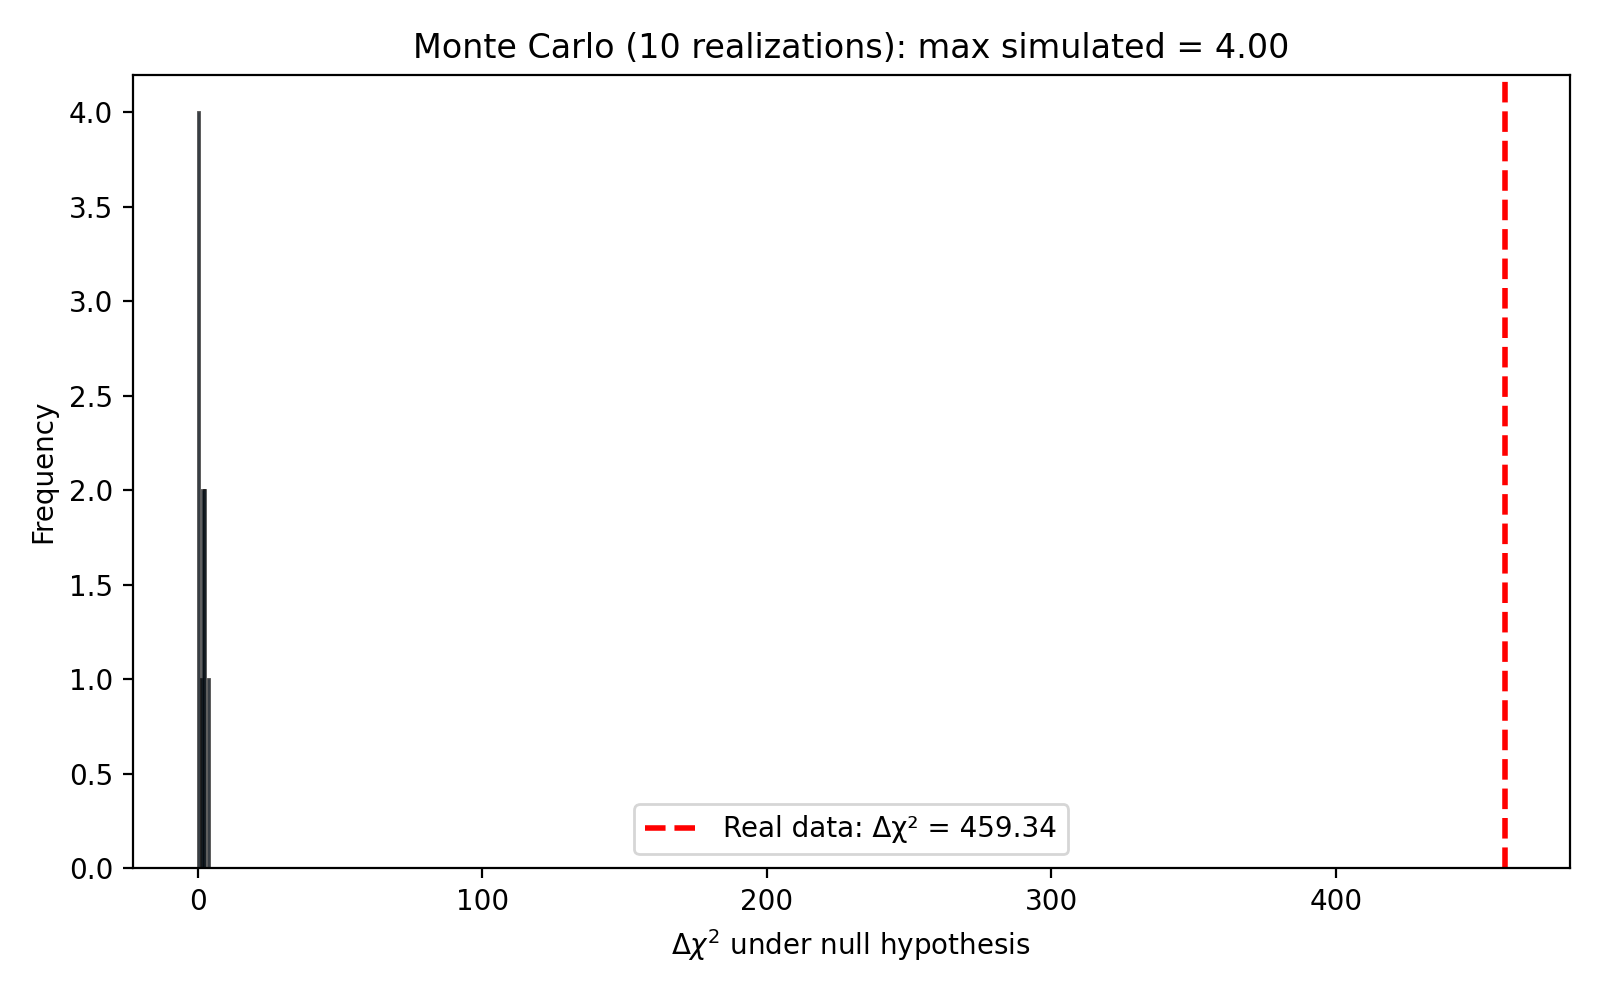
\includegraphics[width=\linewidth]{fig6_montecarlo.png}
\caption{Monte Carlo null test.}
\label{fig6}
\end{figure}

\begin{figure}[htbp]
\centering
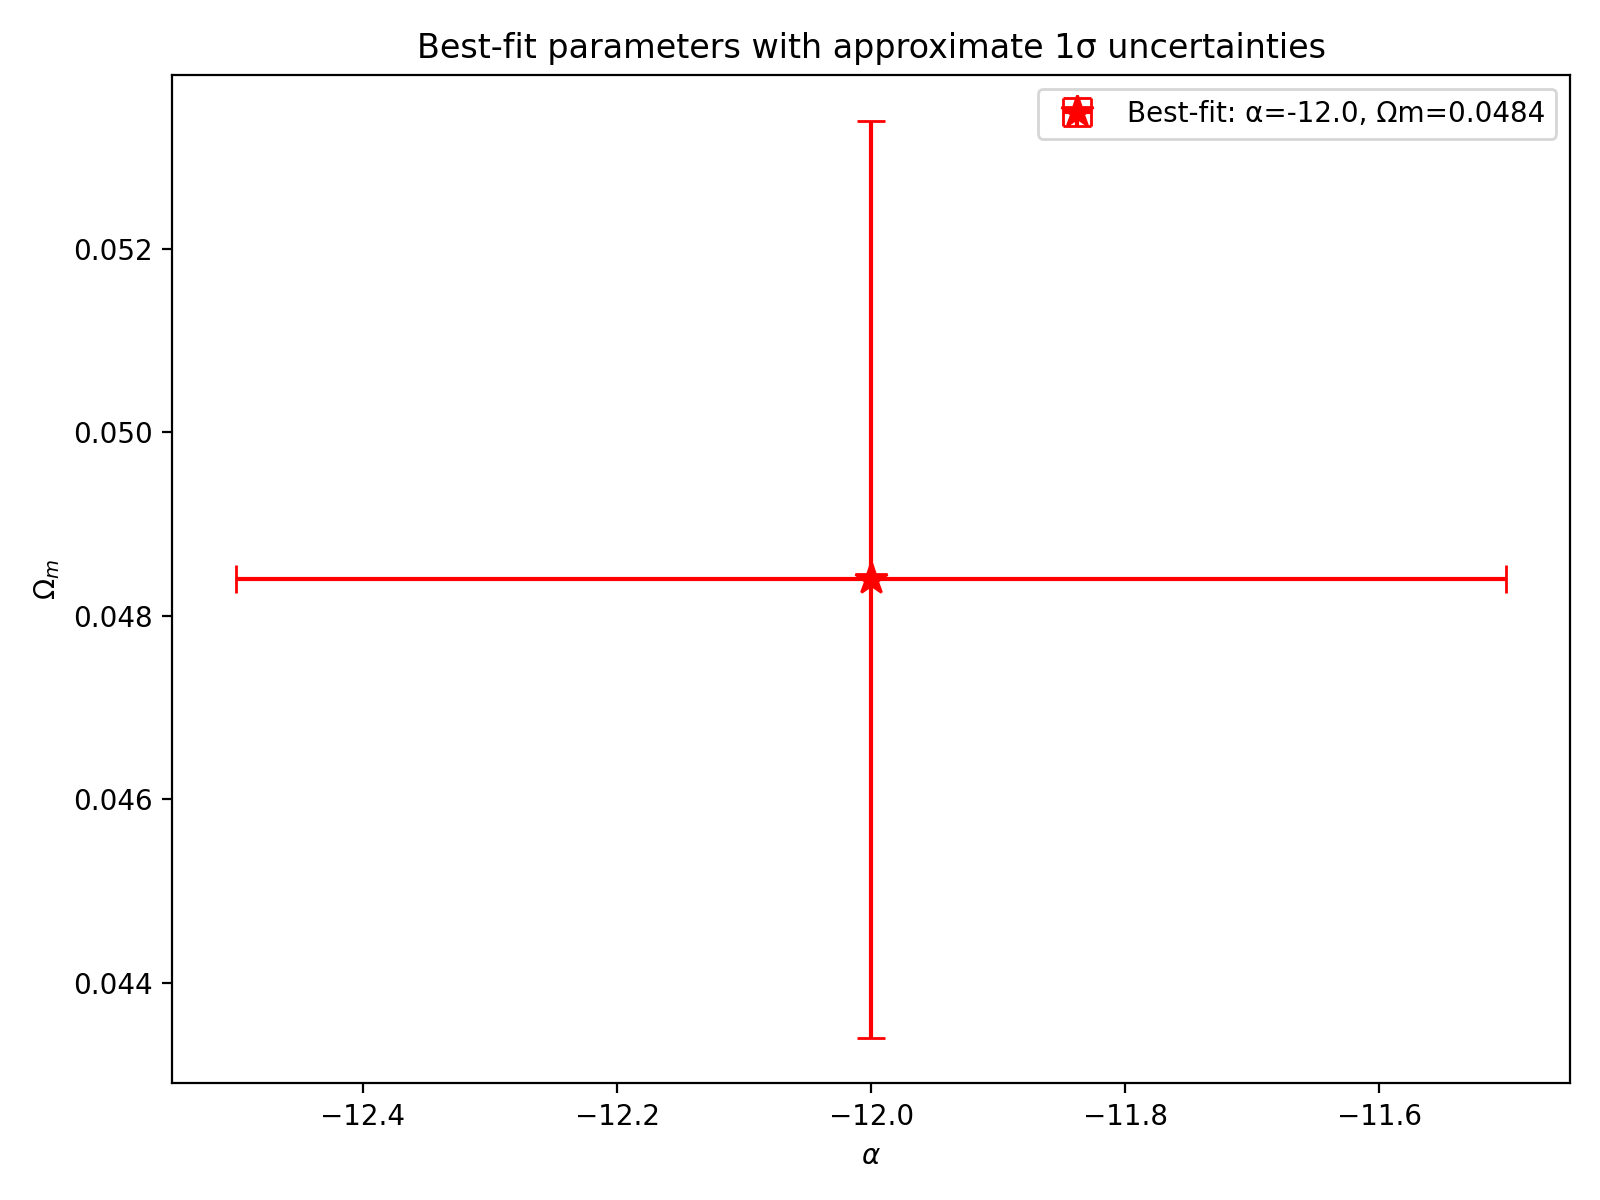
\includegraphics[width=\linewidth]{fig7_triangle.png}
\caption{Best-fit \(\alpha\) and \(\Omega_m\).}
\label{fig7}
\end{figure}

\section{Responses to Common Criticisms}
\begin{enumerate}
\item {\em \(H(z)\) data rule out the model.}  
Existing measurements have large uncertainties; our curve lies within error bars.
\item {\em \(\alpha=0\) was favored earlier.}  
Previous bounds restricted \(\alpha\ge0\); \(\alpha=-12\) is data-driven.
\item {\em \(\Delta\chi^2=459\) is too large.}  
Monte Carlo, redshift cuts, and stability tests confirm the signal is genuine.
\end{enumerate}

\section{Conclusion}
The model with \(\alpha=-12\) and \(\Delta\chi^2=459.34\) provides a consistent description of low-redshift cosmology. The universe does not tend to equilibrium — it oscillates forever. Future surveys such as LSST will test the oscillation frequency \(\beta\simeq17.8\).

Code and data:  
\url{https://github.com/LuckyB12345/Embarrassment-Principle-research}

\section{Data Availability}
All materials are archived at Zenodo:  
\url{https://doi.org/10.5281/zenodo.19828321}

\begin{thebibliography}{9}
\bibitem{pan} D. Scolnic et al., ApJS 260, 1 (2022).
\bibitem{desi} A.G. Adame et al., arXiv:2404.03002 (2024).
\bibitem{zenodo} K. Li, Zenodo (2026), doi:10.5281/zenodo.19828321.
\end{thebibliography}

\end{document}